\documentclass[12pt]{article}

\title{Progetto di sistemi complessi}
\author{Simone Balducci, Alessandro Mancini}
\date{}

\usepackage{amsmath}
\usepackage{amsfonts}
\usepackage{amssymb}
\usepackage{amsthm}
\usepackage{braket}
\usepackage{bbold}
\usepackage[margin=2cm]{geometry}
\usepackage{pgfplots}
\usepackage{fancyhdr}
\usepackage{physics}
\usepackage{systeme,mathtools}
\usepackage{graphicx}
\graphicspath{{./}}
\usepackage{float}
\usepackage{relsize}
\usepackage{dsfont}
\usepackage{calligra}
\usepackage{circuitikz}
\usepackage[miktex]{gnuplottex}
\usepackage{epstopdf}
\usepackage[italian]{babel}
\usepackage{float}
\usepackage[utf8]{inputenc}


\newcommand{\vv}{\vec{v}}
\newcommand{\vw}{\vec{w}}
\newcommand{\vov}{\vec{0_V}}
\newcommand{\vow}{\vec{0_W}}
\newcommand{\vo}{\vec{0}}
\newcommand{\vx}{\vec{x}}
\newcommand{\R}{\Re}
\newcommand{\la}{\lambda}
\newcommand{\bd}{\textbf}
\newcommand{\lang}{\left\langle}
\newcommand{\rang}{\right\rangle}
\newcommand{\lbra}{\left\lbrace}
\newcommand{\rbra}{\right\rbrace}
\newcommand{\ih}{\hat{i}}
\newcommand{\jh}{\hat{j}}
\newcommand{\kh}{\hat{k}}
\newcommand{\nnabla}{\vec{\nabla}}
\newcommand{\vr}{\vec{r}}
\newcommand{\vac}{\vec{a}}
\newcommand{\vf}{\vec{F}}
\newcommand{\vp}{\vec{p}}
\newcommand{\vom}{\vec{\omega}}
\newcommand{\val}{\vec{\alpha}}
\newcommand{\vsr}{\vec{\mathlarger{\mathlarger{\mathlarger{\scriptr}}}}}
\makeatletter
\newcommand*\bigcdot{\mathpalette\bigcdot@{.5}}
\newcommand*\bigcdot@[2]{\mathbin{\vcenter{\hbox{\scalebox{#2}{$\m@th#1\bullet$}}}}}
\makeatother
\def\dbar{{\mathchar'26\mkern-12mu d}}
\DeclareMathAlphabet{\mathcalligra}{T1}{calligra}{m}{n}
\DeclareFontShape{T1}{calligra}{m}{n}{<->s*[2.2]callig15}{}
\newcommand{\scriptr}{\mathcalligra{r}\,}
\newcommand{\boldscriptr}{\pmb{\mathcalligra{r}}\,}

\begin{document}

\maketitle 
\section{L'oscillatore di Van Der Pol}
\subsection{Descrizione}
L'oscillatore di Van Der Pol è un sistema dinamico composto da un oscillatore smorzato, descritto dalla seguente equazione:
\begin{equation}
	\ddot{x} - \mu(1-x^2)\dot{x} + x = 0
\end{equation}
dove $x(t)$ indica l'oscillazione nello spazio delle configurazioni in funzione del tempo e $\mu$ è una costante che indica lo smorzamento. Il termine di mezzo dell'equazione è quello responsabile dello smorzamento, e quindi dell'attrito. 
\begin{figure}[h]
	\centering
	\includegraphics[scale=.4]{Spazio delle fasi oscillatore} 
	\caption{Questa figura mostra traiettorie caratteristiche dell'oscillatore di Van Der Pol nello spazio delle fasi per vari punti iniziali. Si noti anche che l'orientamento del campo vettoriale indirizza tutti i punti materiali verso la stessa traiettoria limite.}
\end{figure}
Si nota subito che nel caso in cui la costante di smorzamento $\mu$ abbia valore nullo, si ottiene un oscillatore armonico classico, e questo verrà verificato nelle sezioni successive mediante simulazioni al computer e esperimenti mediante circuiti elettronici. 
\subsubsection{Studio dell'equazione differenziale}
Consideriamo l'equazione (1) e riscriviamola come:
\begin{equation}
	\ddot{x}+\mu(x^2-1)\dot{x} = \frac{d}{dt}\left(\dot{x}+\mu\left(\frac{1}{3}x^3-x\right)\right) = \frac{d}{dt}\left(\dot{x} + \mu F(x)\right)
\end{equation}
definiamo quindi una nuova variabile
\begin{equation}
	w = \dot{x} + \mu F(x)
\end{equation}
avente derivata 
$$
	\dot{w} = -x
$$
Si ottiene quindi il sistema di equazioni
\begin{equation}
	\begin{cases}
		\dot{x} = w - \mu F(x) \\
		\dot{w} = -x
	\end{cases}
\end{equation}
Studiamo il caso $\dot{x} = 0$, che risulta in
\begin{equation}
	w(x) = \mu F(x) = \mu\left(\frac{1}{3}x^3-x\right)
\end{equation}
e si ottiene quindi una cubica. Studiamo quindi il grafico di questa funzione: 
\begin{figure}[H]
	\centering
	\input{VecField.tex}
\end{figure}
Vediamo che $\dot{w} = 0$ solo per $x=0$, ovvero quando siamo sull'asse delle $y$, e si trova in particolare che sopra l'asse delle $x$ i vettori del campo vettoriale puntano a destra, mentre sotto l'asse delle $x$ puntano a sinistra. Il punto di massimo locale della funzione è $\left(-1,\frac{2}{3}\mu\right)$, mentre il punto di minimo locale è $\left(1,-\frac{2}{3}\mu\right)$. In più vediamo che i punti di intersezione tra le orizzontali che passano per i punti di massimo e minimo con la curva $w$ sono rispettivamente $\left(2,\frac{2}{3}\mu\right)$ $\left(-2,-\frac{2}{3}\mu\right)$. \\
Se consideriamo valori di $\mu$ molto più grandi di 1, vediamo che sarebbe ragionevole riscalare di nuovo le variabili:
\begin{equation}
	y = \frac{w}{\mu} \ \ \Longrightarrow \ \ \begin{cases}
		\dot{x} = \mu(y - F(x)) \\
		\dot{y} = -\frac{1}{\mu}x	
	\end{cases}
\end{equation}
Così si ottiene un grafico uguale a quello di prima ma senza i valori di $\mu$. \\
Fuori dalla curva $\dot{x} = 0$ si ha che $\dot{x}$ è molto grande, mentre $\dot{y}$ è quasi nullo. Questo vuole dire che se mettiamo una particella fuori dalla curva, questa verrà spostata orizzontalmente molto velocemente fino a posizionarsi sulla curva, e subirà anche una piccola accelerazione verticale nella direzione verso la curva. A questo punto la particella si muoverà lentamente sulla curva fino a uno dei vue punti critici, e una volta raggiunti accelererà molto velocemente fino al secondo, in corrispondenza del quale si muoverà molto più lentamente. \\
Si ottiene così un ciclo limite in cui la velocità della particella varia continuamente. In particolare notiamo che più il valore di $\mu$ è grande, più la curva si muoverà lentamente vicino ai punti di minimo/massimo e velocemente lontano da essi. Questo spiega la forma delle traiettorie viste nelle figure $$ a $$ e sarà inoltre dimostrato visivamente con delle animazioni.
\subsubsection{Studio della stabilità }
Per studiare la stabilità dell'oscillatore di Van Der Pol e la dipendenza della stessa dalla costante di smorzamento $\mu$, si usa il metodo di Lyapunov: \\ \\
\textbf{Primo teorema di Lyapunov: \\}
Per un sistema descritto da un'equazione del tipo 
\begin{equation}
	\dot{\vec{x}} = f(\vec{x},t)
\end{equation}
dove $f(\vo,t) = \vo$ per tutti i $t \geq t_0$, se esiste una funzione scalare $V(\vec{x},t)$ avente derivate parziali continue e che sottisfa le condizioni: 

1) $V(\vec{x},t)$ è definita positiva. 

2) $\dot{V}(\vec{x},t)$ è definita negativa. \\
allora il punto di equilibrio è stabile asintoticamente. \\ \\
Applichiamo ora questo teorema al caso dell'oscillatore di Van Der Pol.  \\
Prima di tutto definiamo una nuova variabile $y = \dot{x}$, in modo da passare da una singola equazione differenziale di secondo ordine a un sistema di due equazioni di primo ordine:
\begin{equation}
	\begin{cases}
		y = \dot{x} \\
		\dot{y} = \mu(1-x^2)y - x
	\end{cases}
\end{equation}
Queste equazioni rappresentano le equazioni del moto dell'oscillatore nello spazio della fasi e possono essere usate per trovare numericamente le traiettorie limite, come si vedrà nella sezione 2. \\
Consideriamo ora una funzione $V(\vec{x},t)$ del tipo 
\begin{equation}
	V(\vec{x},t) = \frac{1}{2}(x^2 + y^2)
\end{equation}
Questa funzione rispetta la prima caratteristica richiesta dal teorema di Lyapunov, ovvero è definita positiva. Si nota che la costante $1/2$ non era strettamente necessaria, ma è stata aggiunta perchè facendo la derivata totale rispetto al tempo di $V$, questa costante si semplifica e si ritrova il termine dissipativo dell'equazione (1). \\
Ora calcoliamo la derivata della funzione $V$:
$$
	\dot{V}(\vec{x},t) = x\dot{x} + y\dot{y} = x\dot{x} + \mu(1-x^2)\dot{x}^2-x\dot{x} = \mu(1-x^2)\dot{x}^2
$$
\begin{equation}
	\dot{V}(\vec{x},t) = \mu(1-x^2)\dot{x}^2
\end{equation}
Vediamo che in prossimità dell'origine questa funzione è definita negativa se e solo se $\mu$ è negativo. \\
Ne concludiamo quindi che per valori negativi di $\mu$ l'origine è un punto di equilibrio asintotico, e si dice quindi punto attrattivo. \\
Dallo studio della stabilità dell'oscillatore con il metodo di Lyapunov si trova che: 

-Se $\mu>0$, si ha che l'origine è un punto instabile e la particella si allontana da esso, fino ad arrivare su una traiettoria limite che è stabile. Si dice quindi che quella traiettoria è attrattiva. 

-Se $\mu<0$, si ha che l'origine è un punto attrattivo, quindi le traiettorie subiscono una degenerazione attorno ad essa. \\
\begin{center}
	\includegraphics[scale=0.7]{Traiettorie}
\end{center}
Per valori di $\mu$ positivi, ovvero per cui si hanno delle traiettorie limite che attraggono i punti nello spazio delle fasi, si nota che l'ambiezza di queste curve cresce con lo smorzamento. \\
Come accennato in precedenza, nel caso particolare in cui $\mu = 0$, il sistema si riduce a un oscillatore armonico, quindi la traiettoria sarà una circonferenza.
\begin{center}
	\includegraphics[scale=1]{Vari smorzamenti} 
\end{center}
\subsection{Storia}
L'oscillatore di Van Der Pol è stato ideato originariamente dall'ingegnere elettrico olandese Balthasar Van Der Pol. Van Der Pol scoprì delle oscillazioni stabili, che in seguito chiamò rilassamento-oscillazioni e che sono un tipo ci ciclo limite nei circuiti elettrici che utilizzano i vacuum tubes. \\
Quando questi circuiti venivano portati vicino al ciclo limite,. \\
Van Der Pol e i suoi colleghi scoprirono inoltre che a certe frequenze si sentiva un rumore irregolare, che più avanti verrà attribuito al caos deterministico. 
\subsection{Applicazioni}
\subsubsection{Il neurone \\}
\subsubsection{Il modello di Fitzhugh-Nagumo}
La caratteristica più importante di un neurone è la sua eccitabilità, cioè la sua capacità di depolarizzarsi e ripolarizzarsi velocemente rispetto al potenziale di membrana a riposo, producendo così un picco stretto noto come potenziale d'azione. Il potenziale di membrana è la differenza di potenziale elettrico tra l'interno e l'esterno della membrana cellulare. \\ \\
Il miglior modello per descrivere la dinamica di un neurone eccitato il il modello di Hodgkin-Huxley. Tuttavia, nonostante questo modello sia molto preciso da un punto di vista fisiologico, esso ha diversi difetti di tipo pratico. In particolare, essendo un modello altamente non lineare, può esibire molti comportamenti caotici, che sono difficili da studiare in quattro dimensioni. Per questo motivo spesso si studia il modello di FitzHugh-Nagumo, che è più semplice e facilmente studiabile. Infatti questo modello può essere visto come la proiezione bidimensionale del modello di Hodgkin-Huxley. \\ \\
La dinamica del modello di Fitzhugh-Nagumo è descritta da un sistema di equazioni differenziali non lineari, caratterizzate dalla presenza di due scale temporali:
\begin{equation}
	\begin{cases}
		\varepsilon\dot{u}(t) = u(t) - \frac{u^3(t)}{3}-v(t)+I_{e}(t) \\
		\dot{v}(t) = u(t) + a
	\end{cases}
\end{equation}
La $u(t)$ rappresenta la variabile veloce, ovvero la variabile che cambia più velocemente, che presenta una dinamica piccata di quasi-soglia, simile al potenziale di membrana. La $v(t)$ è la variabile lenta, che si chiama variabile di recupero, e rappresenta la caratteristica refrattarietà del neurone dopo essersi eccitato. La separazione tra le due scale temporali è dettata dal parametro $\varepsilon$. $I_e$ è uno stimolo esterno, che può rappresentare le correnti date dalle interazioni con gli altri neuroni o dagli stimoli esterni. Infine $a$ è un parametro dinamico che regola il regime dinamico del modello. \\ \\
Il sistema possiede un punto fisso $(u,v) = \left(-a,-a+\frac{a^3}{3} \right) $ che è stabile quando $|a|>1$ e diventa instabile quando $|a|<1$, e in questa condizione si presenta un ciclo limite. \\
Il primo regime dinamico si chiama eccitabile, che è interpretabile come un neurone standard, mentre il secondo regime è il regime di "spiking tonico", che può essere interpretato come un neurone pacemaker.Per capire il meccanismo della produzione dei picchi analizziamo lo spazio delle fasi. Disegnamo le nullcline, ovvero le curve lungo le quali le derivate temporali delle rispettive variabili temporali sono nulle. La nullclina della variabile $v$ quindi è una curva verticale in $u = -a$, mentre la nullclina di $u$ è una cubila. \\
Nel regime di spiking tonico, il ciclo limite è composto da quattro fasi:

1) Un lento moto in alto lungo il ramo destro della nullclina. 

2) Un veloce salto verso il ramo sinistro.

3) Un lento moto verso il basso lungo il ramo sinistro. 

4) Un veloce salto verso il ramo sinistro.\\ \\
Nella fase di attività tonica questi stati sono ripetuti indefinitamente. \\
Nello stato eccitabile, il punto fisso diventa attrattivo, e il sistema non perturbato tende a raggiungerlo muovendoli lungo la nullclina cubica. \\
Se ad esempio prendiamo $a > 1$, il punto fisso si troverà sul ramo sinistro della nullclina cubica. Se applichiamo un veloce shock positivo mediante la variabile $I_e$, il sistema si sposterà verso la direzione positiva delle $u$, e in base all'entità dello shock possono succedere due fenomeni: Se l'impulso è sotto il livello di soglia, il sistema verrà ricatturato dal ramo refrattario e continuerà a muoversi asintoticamente verso il punto fisso. Se invece l'impulso è sopra il livello di soglia, il sistema salterà verso la regione attiva, seguendola fino a raggiungere un massimo in $u = 1$, e a quel punto salterà indietro verso il ramo refrattario, riprendendo il moto asintotico. Quest'ultimo effetto prende il nome di effetto di quasi-soglia.


  
\subsection{Varianti: L'oscillatore di Van Der Pol forzato}

\section{Soluzione numerica e simulazione}
Per risolvere l'equazione differenziale dell'oscillatore è stato scritto un codice in C++, che ha permesso di trovare i valori di $x$ per dei valori di tempo discretizzati $t = n\Delta$. Per fare ciò si è partiti dall'equazione 2, ma per permettere al computer di interpretarla la si è dovuta discretizzare, ottenendo il seguente sistema:
\begin{equation}
	\begin{cases}
	x_{n+1} = x_n + y_n\Delta \\
	y_{n+1} = y_n + \left(\mu(1-x_n^2)y_n - x_n\right)\Delta
	\end{cases}
\end{equation} 
Sulla base di questo sistema di equazioni discretizzate è stato quindi scritto il seguente codice: \\ \\ \\
Come di vede, questo codice prende come parametri di entrata le coordinate iniziali $x_0$ e $y_0$, il parametro di smorzamento $\mu$ e lo step temporale $\Delta$. L'ultimo parametro è il tempo $t$, e scegliendo questo valore si ottengono i valori della $x$ per ogni istante temporale precedente al $t$ scelto. \\
	Mediante questo codice vogliamo osservare certe caratteristiche dell'oscillatore: \\
1) Vogliamo osservare la traiettoria caratteristica di un punto nello spazio delle fasi. \\
2) Vogliamo confrontare traiettorie diverse con stesse coordinate iniziali ma con diversi valori del parametro di smorzamento. \\
3) Vogliamo osservare un comportamento particolare del modello di Van Der Pol, ovvero che se prendiamo un insieme di tanti punti distribuiti in modo casuale nello spazio delle fasi, dopo poche iterazioni questi seguono tutti la stessa traiettoria, che è quindi una curva attrattrice. \\
4) Vogliamo infine osservare l'andamento temporale della posizione $x$ della particella. \\
Partiamo dal primo obiettivo, ovvero la traiettoria carattestistica: 
\begin{figure}[H]
	\centering
	\scalebox{0.9}{% GNUPLOT: LaTeX picture with Postscript
\begingroup
  % Encoding inside the plot.  In the header of your document, this encoding
  % should to defined, e.g., by using
  % \usepackage[cp1252,<other encodings>]{inputenc}
  \inputencoding{cp1252}%
  \makeatletter
  \providecommand\color[2][]{%
    \GenericError{(gnuplot) \space\space\space\@spaces}{%
      Package color not loaded in conjunction with
      terminal option `colourtext'%
    }{See the gnuplot documentation for explanation.%
    }{Either use 'blacktext' in gnuplot or load the package
      color.sty in LaTeX.}%
    \renewcommand\color[2][]{}%
  }%
  \providecommand\includegraphics[2][]{%
    \GenericError{(gnuplot) \space\space\space\@spaces}{%
      Package graphicx or graphics not loaded%
    }{See the gnuplot documentation for explanation.%
    }{The gnuplot epslatex terminal needs graphicx.sty or graphics.sty.}%
    \renewcommand\includegraphics[2][]{}%
  }%
  \providecommand\rotatebox[2]{#2}%
  \@ifundefined{ifGPcolor}{%
    \newif\ifGPcolor
    \GPcolortrue
  }{}%
  \@ifundefined{ifGPblacktext}{%
    \newif\ifGPblacktext
    \GPblacktextfalse
  }{}%
  % define a \g@addto@macro without @ in the name:
  \let\gplgaddtomacro\g@addto@macro
  % define empty templates for all commands taking text:
  \gdef\gplbacktext{}%
  \gdef\gplfronttext{}%
  \makeatother
  \ifGPblacktext
    % no textcolor at all
    \def\colorrgb#1{}%
    \def\colorgray#1{}%
  \else
    % gray or color?
    \ifGPcolor
      \def\colorrgb#1{\color[rgb]{#1}}%
      \def\colorgray#1{\color[gray]{#1}}%
      \expandafter\def\csname LTw\endcsname{\color{white}}%
      \expandafter\def\csname LTb\endcsname{\color{black}}%
      \expandafter\def\csname LTa\endcsname{\color{black}}%
      \expandafter\def\csname LT0\endcsname{\color[rgb]{1,0,0}}%
      \expandafter\def\csname LT1\endcsname{\color[rgb]{0,1,0}}%
      \expandafter\def\csname LT2\endcsname{\color[rgb]{0,0,1}}%
      \expandafter\def\csname LT3\endcsname{\color[rgb]{1,0,1}}%
      \expandafter\def\csname LT4\endcsname{\color[rgb]{0,1,1}}%
      \expandafter\def\csname LT5\endcsname{\color[rgb]{1,1,0}}%
      \expandafter\def\csname LT6\endcsname{\color[rgb]{0,0,0}}%
      \expandafter\def\csname LT7\endcsname{\color[rgb]{1,0.3,0}}%
      \expandafter\def\csname LT8\endcsname{\color[rgb]{0.5,0.5,0.5}}%
    \else
      % gray
      \def\colorrgb#1{\color{black}}%
      \def\colorgray#1{\color[gray]{#1}}%
      \expandafter\def\csname LTw\endcsname{\color{white}}%
      \expandafter\def\csname LTb\endcsname{\color{black}}%
      \expandafter\def\csname LTa\endcsname{\color{black}}%
      \expandafter\def\csname LT0\endcsname{\color{black}}%
      \expandafter\def\csname LT1\endcsname{\color{black}}%
      \expandafter\def\csname LT2\endcsname{\color{black}}%
      \expandafter\def\csname LT3\endcsname{\color{black}}%
      \expandafter\def\csname LT4\endcsname{\color{black}}%
      \expandafter\def\csname LT5\endcsname{\color{black}}%
      \expandafter\def\csname LT6\endcsname{\color{black}}%
      \expandafter\def\csname LT7\endcsname{\color{black}}%
      \expandafter\def\csname LT8\endcsname{\color{black}}%
    \fi
  \fi
    \setlength{\unitlength}{0.0500bp}%
    \ifx\gptboxheight\undefined%
      \newlength{\gptboxheight}%
      \newlength{\gptboxwidth}%
      \newsavebox{\gptboxtext}%
    \fi%
    \setlength{\fboxrule}{0.5pt}%
    \setlength{\fboxsep}{1pt}%
    \definecolor{tbcol}{rgb}{1,1,1}%
\begin{picture}(6802.00,6802.00)%
    \gplgaddtomacro\gplbacktext{%
      \csname LTb\endcsname%%
      \put(682,704){\makebox(0,0)[r]{\strut{}$-4$}}%
      \put(682,1439){\makebox(0,0)[r]{\strut{}$-3$}}%
      \put(682,2173){\makebox(0,0)[r]{\strut{}$-2$}}%
      \put(682,2908){\makebox(0,0)[r]{\strut{}$-1$}}%
      \put(682,3643){\makebox(0,0)[r]{\strut{}$0$}}%
      \put(682,4377){\makebox(0,0)[r]{\strut{}$1$}}%
      \put(682,5112){\makebox(0,0)[r]{\strut{}$2$}}%
      \put(682,5846){\makebox(0,0)[r]{\strut{}$3$}}%
      \put(682,6581){\makebox(0,0)[r]{\strut{}$4$}}%
      \put(814,484){\makebox(0,0){\strut{}$-2.5$}}%
      \put(1373,484){\makebox(0,0){\strut{}$-2$}}%
      \put(1932,484){\makebox(0,0){\strut{}$-1.5$}}%
      \put(2491,484){\makebox(0,0){\strut{}$-1$}}%
      \put(3050,484){\makebox(0,0){\strut{}$-0.5$}}%
      \put(3610,484){\makebox(0,0){\strut{}$0$}}%
      \put(4169,484){\makebox(0,0){\strut{}$0.5$}}%
      \put(4728,484){\makebox(0,0){\strut{}$1$}}%
      \put(5287,484){\makebox(0,0){\strut{}$1.5$}}%
      \put(5846,484){\makebox(0,0){\strut{}$2$}}%
      \put(6405,484){\makebox(0,0){\strut{}$2.5$}}%
    }%
    \gplgaddtomacro\gplfronttext{%
      \csname LTb\endcsname%%
      \put(209,3642){\rotatebox{-270}{\makebox(0,0){\strut{}p}}}%
      \put(3609,154){\makebox(0,0){\strut{}x}}%
    }%
    \gplbacktext
    \put(0,0){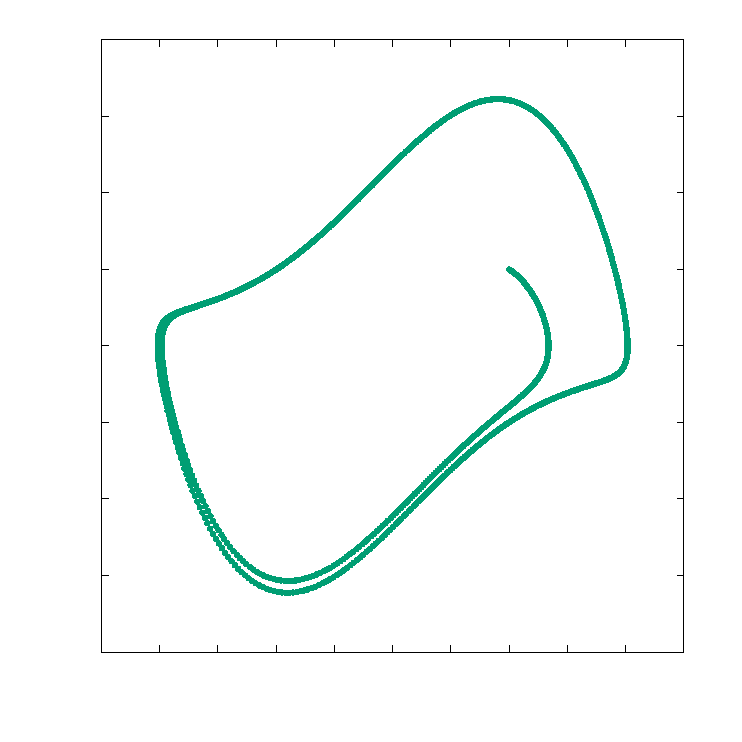
\includegraphics[width={340.10bp},height={340.10bp}]{Schema1-5}}%
    \gplfronttext
  \end{picture}%
\endgroup
}
\end{figure}
Nella figura soprastante si può vedere la traiettoria caratteristica dell'oscillatore di Van Der Pol. Come è stato spiegato nelle sezioni precedenti, la velocità del punto che si muove secondo questa traiettoria non è affatto costante.
Come si può notare dall'animazione infatti, il punto si muove molto più velocemente nei lati corti della traiettoria e più lentamente nei lati lunghi. Si avrà quindi un accumulo di punti in corrispondenza dei punti in cui il momento cambia segno,
che nel grafico soprastante si trovano in corrispondenza dei punti $(-2,0)$ e $(2,0)$ approssimativamente. \\
Nell'immagine sottostante si può vedere uno degli ultimi frame dell'animazione citata in precedenza e si vede chiaramente che nei lati corti si hanno degli accumuli di punti, mentre lungo i lati lunghi i punti si distribuiscono in maniera molto meno densa. 
\begin{figure}[H]
	\centering
	\input{LastFrame.tex}
\end{figure}
Vogliamo ora confrontare le traiettorie di particelle aventi stesse coordinate iniziali ma diverse costanti di smorzamento. \\
Ci aspettiamo che il grafico ottenuto dalla simulazione numerica sia simile a quello visto in figura $$ afads $$. Dalla simulazione si ottiene il seguente grafico: \\ \\ \\ \\ \\
che riporta l'andamento atteso. Studiamo questo grafico: \\
La cosa principale che si nota è che, con l'aumentare del valore di $\mu$, la traiettoria si allunga e assume una forma pià angolata. Il motivo di questo comportamento è stato spiegato nella sezione precedente e deriva dallo studio dell'equazione differenziale. \\
Vogliamo ora considerare le traiettorie in corrispondenza di valori piccoli di $\mu$. 
\begin{figure}[H]
	\centering
	\input{Collasso.tex}
\end{figure}
Nel grafico soprastante si vede che la particella parte vicino all'origine e viene attratta verso essa, percorrendo quindi delle orbite che degenerano fino a collassare in un punto.
Vogliamo ora studiare un comportamento molto interessante di questo tipo di oscillatore che è stato accennato nelle pagine precedenti. \\
Consideriamo una situazioni iniziale come quella nel grafico seguente 
\begin{figure}[H]
	\centering
	\input{FirstFrame.tex}
\end{figure}
quindi una situazione in cui abbiamo un grande numero di punti (in questo caso ne sono stati plottati 300) che sono distribuiti randomicamente nello spazio delle fasi, quindi con momento iniziale e coordinata $x$ iniziale randomici. \\
Se lasciamo partire questi punti, sembra inizialmente che questi si muovano in modo caotico, ma dopo una decina di iterazioni si vede che le particelle stanno in realtà andando a formare una stessa traiettoria, che è la traiettoria caratteristica dell'oscillatore di Van Der Pol. \\
In base alla loro posizione iniziale i punti ci metteranno più o meno tempo a posizionarsi su questa curva, ma dopo un numero sufficientemente grande di iterazioni (nella simulazione considerata sono servite circa 350 iterazioni) tutti i punti si saranno posizionati sulla curva. \\
Questo comportamento peculiare è un'altra dimostrazione del fatto che la traiettoria dell'oscillatore di Van Der Pol sia una curva attrattiva. \\ \\
Infine si vuole studiare l'andamento temporale della $x$. 
\begin{figure}[H]
	\input{AndTemp.tex}
\end{figure}
Nella figura soprastante si vede che l'andamento della $x$ ricorda vagamente una sinusoide, per la periodicità, ma ha una forma molto più aguzza. Si nota inoltre che la forma della funzione tra un punto di minimo e un punto di massimo e viceverda mantiene la stessa forma, ma risulta capovolta. \\
Si nota inoltre che la forma della funzione tra un punto di minimo e un punto di massimo e viceverda mantiene la stessa forma, ma risulta capovolta. \\
La forma di queste oscillazioni cambia molto con il valore della costante di smorzamento. Infatti si trova che per valori più piccoli di $\mu$ le oscillazioni hanno una forma più aguzza, mentre per valori grandi (da circa 5 in su) l'andamento ha una forma più squadrata. \\
Per rendere l'idea in un modo tutt'altro che rigoroso, per valori piccoli di $\mu$ l'andamento ha una forma che ricorda il dente di un lupo, mentre per valori grandi ha una forma che ricorda il dente di uno squalo. \\ \\ 
Questo è l'andamento temporale nel caso dell'oscillatore non forzato. \\
Per un oscillatore forzato si troverebbe un andamento vagamente simile a questo, ma con una forma molto più irregolare. Questo è dovuto al fatto che in un'oscillatore del genere, una forzante periodica producerebbe una caoticità, che renderebbe quindi molto più imprevedibile la traiettoria.
\subsection{Equazioni rigide e ordine di accuratezza}
Un'equazione differenziale si dice rigida (o stiff) quando certi di metodi di soluzione sono numericamente instabili a meno che il passo d'integrazione sia preso estremamente piccolo. L'idea generale della definizione di rigidità è che l'equazione includa dei termini che possono portare a rapide variazioni delle soluzioni. \\ \\
In questo caso è utile anche introdurre il concetto di ordine di accuratezza di una soluzione numerica. \\
L'ordine di accuratezza quantifica il tasso di convergenza della soluzione approssimata dell'equazione differenziale alla sua soluzione esatta. \\
Stiamo parlando di funzioni, quindi ci posizioniamo in uno spazio normato di funzioni $(V,||\cdot||)$, dove la norma deve essere scelta opportunamente, e si considera che l'equazione abbia una soluzione esatta $v$ e una soluzione numerica approssimata $v_h$, dove $h$ è il parametro che caratterizza l'approssimazione, quindi il time step. \\
A questo punto si dice che la soluzione $v_h$ ha un'accuratezza di ordine n se l'errore
\begin{equation}
	E(h) = ||v-v_h|| \leq Ch
\end{equation}
dove $C$ è una costante indipendente da $h$ che dipende solo dalla soluzione $v$. \\
Possiamo esprimere questo concetto con la notazione degli O-grandi:
\begin{equation}
	||v-v_h|| = O(h^n)
\end{equation}
Questa definizione dipende fortemente dalla norma usata nello spazio $V$, e quindi la scelta di questa norma è essenziale per calcolare correttamente il tasso di convergenza delle soluzioni approssimate. \\ \\
L'equazione di Van Der Pol è un'equazione che cade nella definizione di equazione rigida, quindi per risolverla correttamente è essenziale scegliere dei time-step abbastanza piccoli. La rigidità (stiffness) di quest'equazione è contenuta nella costante $\mu$, e questo può essere visualizzato confrontando le soluzioni ottenute variando i time step. Per fare ciò confrontiamo prima gli andamenti temporali delle $x$ e delle $p$, e in seguito le traiettorie nello spazio delle fasi, per valori di $\mu$ dell'ordine dell'unità, e in seguito alziamo il valore di $\mu$ e rifacciamo questo confronto, per verificare come cambino i risultati.
\subsubsection{Confronto sulla rigidità per $\mu = 1$}
Come detto, il parametro $\mu$ determina la rigidità dell'equazione di Van Der Pol, quindi per $\mu = 1$ l'equazione sarà poco rigida, e ne risulta che si potranno ottenere soluzioni accurate con tipe step non eccessivamente brevi. \\ \\
Confrontando i risultati con le soluzioni "esatte" trovate in rete si è notato che con questa rigidità, si può ottenere una soluzione quasi identica alla soluzione "esatta" utilizzando un time step di $h = 10^{-4}$, quindi si è preso questo valore come riferimento e si sono considerate le traiettorie ottenute mediante esso come esatte. \\ \\
Confrontiamo prima l'andamento temporale della $x(t)$. Questo confronto viene fatto per $\Delta t = 0.1$, $\Delta t = 0.01$ e $\Delta t = 0.001$. Si è provato anche a usare un timestep $h=1$, ma la soluzione è risultata altamente instabile, a indicare che questo valore sia troppo piccolo per risolvere quest'equazione. 
\begin{figure}[H]
	\centering
	\scalebox{0.9}{\input{ConfrXGGG.tex}}
\end{figure}
\begin{figure}[H]
	\centering
	\input{ConfrXZ.tex}
\end{figure}
Come si può vedere nel grafico soprastante, per $\Delta t = 0.001$ si ottiene una curva quasi identica a quella considerata esatta, per $\Delta t = 0.01$ si ottiene una curva molto molto simile mentre per $\Delta t = 0.1$ si ottiene una curva decisamente diversa, ad indicare che questo time step è troppo lungo per risolvere l'equazione con questo grado di rigidità in maniera precisa e soddisfacente. \\
Nel grafico soprastante si può vedere uno zoom del grafico precedente, che permette di osservare che le curve verdi e viola siano effettivamente quasi identiche, infatti sono quasi completamente sovrapposte. \\
Ora confrontiamo l'andamento temporale di $p(t)$: 
\begin{figure}[H]
	\centering
	% GNUPLOT: LaTeX picture with Postscript
\begingroup
  % Encoding inside the plot.  In the header of your document, this encoding
  % should to defined, e.g., by using
  % \usepackage[cp1252,<other encodings>]{inputenc}
  \inputencoding{cp1252}%
  \makeatletter
  \providecommand\color[2][]{%
    \GenericError{(gnuplot) \space\space\space\@spaces}{%
      Package color not loaded in conjunction with
      terminal option `colourtext'%
    }{See the gnuplot documentation for explanation.%
    }{Either use 'blacktext' in gnuplot or load the package
      color.sty in LaTeX.}%
    \renewcommand\color[2][]{}%
  }%
  \providecommand\includegraphics[2][]{%
    \GenericError{(gnuplot) \space\space\space\@spaces}{%
      Package graphicx or graphics not loaded%
    }{See the gnuplot documentation for explanation.%
    }{The gnuplot epslatex terminal needs graphicx.sty or graphics.sty.}%
    \renewcommand\includegraphics[2][]{}%
  }%
  \providecommand\rotatebox[2]{#2}%
  \@ifundefined{ifGPcolor}{%
    \newif\ifGPcolor
    \GPcolortrue
  }{}%
  \@ifundefined{ifGPblacktext}{%
    \newif\ifGPblacktext
    \GPblacktextfalse
  }{}%
  % define a \g@addto@macro without @ in the name:
  \let\gplgaddtomacro\g@addto@macro
  % define empty templates for all commands taking text:
  \gdef\gplbacktext{}%
  \gdef\gplfronttext{}%
  \makeatother
  \ifGPblacktext
    % no textcolor at all
    \def\colorrgb#1{}%
    \def\colorgray#1{}%
  \else
    % gray or color?
    \ifGPcolor
      \def\colorrgb#1{\color[rgb]{#1}}%
      \def\colorgray#1{\color[gray]{#1}}%
      \expandafter\def\csname LTw\endcsname{\color{white}}%
      \expandafter\def\csname LTb\endcsname{\color{black}}%
      \expandafter\def\csname LTa\endcsname{\color{black}}%
      \expandafter\def\csname LT0\endcsname{\color[rgb]{1,0,0}}%
      \expandafter\def\csname LT1\endcsname{\color[rgb]{0,1,0}}%
      \expandafter\def\csname LT2\endcsname{\color[rgb]{0,0,1}}%
      \expandafter\def\csname LT3\endcsname{\color[rgb]{1,0,1}}%
      \expandafter\def\csname LT4\endcsname{\color[rgb]{0,1,1}}%
      \expandafter\def\csname LT5\endcsname{\color[rgb]{1,1,0}}%
      \expandafter\def\csname LT6\endcsname{\color[rgb]{0,0,0}}%
      \expandafter\def\csname LT7\endcsname{\color[rgb]{1,0.3,0}}%
      \expandafter\def\csname LT8\endcsname{\color[rgb]{0.5,0.5,0.5}}%
    \else
      % gray
      \def\colorrgb#1{\color{black}}%
      \def\colorgray#1{\color[gray]{#1}}%
      \expandafter\def\csname LTw\endcsname{\color{white}}%
      \expandafter\def\csname LTb\endcsname{\color{black}}%
      \expandafter\def\csname LTa\endcsname{\color{black}}%
      \expandafter\def\csname LT0\endcsname{\color{black}}%
      \expandafter\def\csname LT1\endcsname{\color{black}}%
      \expandafter\def\csname LT2\endcsname{\color{black}}%
      \expandafter\def\csname LT3\endcsname{\color{black}}%
      \expandafter\def\csname LT4\endcsname{\color{black}}%
      \expandafter\def\csname LT5\endcsname{\color{black}}%
      \expandafter\def\csname LT6\endcsname{\color{black}}%
      \expandafter\def\csname LT7\endcsname{\color{black}}%
      \expandafter\def\csname LT8\endcsname{\color{black}}%
    \fi
  \fi
    \setlength{\unitlength}{0.0500bp}%
    \ifx\gptboxheight\undefined%
      \newlength{\gptboxheight}%
      \newlength{\gptboxwidth}%
      \newsavebox{\gptboxtext}%
    \fi%
    \setlength{\fboxrule}{0.5pt}%
    \setlength{\fboxsep}{1pt}%
    \definecolor{tbcol}{rgb}{1,1,1}%
\begin{picture}(10204.00,5668.00)%
    \gplgaddtomacro\gplbacktext{%
      \csname LTb\endcsname%%
      \put(682,704){\makebox(0,0)[r]{\strut{}$-3$}}%
      \put(682,1495){\makebox(0,0)[r]{\strut{}$-2$}}%
      \put(682,2285){\makebox(0,0)[r]{\strut{}$-1$}}%
      \put(682,3076){\makebox(0,0)[r]{\strut{}$0$}}%
      \put(682,3866){\makebox(0,0)[r]{\strut{}$1$}}%
      \put(682,4657){\makebox(0,0)[r]{\strut{}$2$}}%
      \put(682,5447){\makebox(0,0)[r]{\strut{}$3$}}%
      \put(814,484){\makebox(0,0){\strut{}$0$}}%
      \put(1394,484){\makebox(0,0){\strut{}$1$}}%
      \put(1974,484){\makebox(0,0){\strut{}$2$}}%
      \put(2555,484){\makebox(0,0){\strut{}$3$}}%
      \put(3135,484){\makebox(0,0){\strut{}$4$}}%
      \put(3715,484){\makebox(0,0){\strut{}$5$}}%
      \put(4295,484){\makebox(0,0){\strut{}$6$}}%
      \put(4875,484){\makebox(0,0){\strut{}$7$}}%
      \put(5456,484){\makebox(0,0){\strut{}$8$}}%
      \put(6036,484){\makebox(0,0){\strut{}$9$}}%
      \put(6616,484){\makebox(0,0){\strut{}$10$}}%
      \put(7196,484){\makebox(0,0){\strut{}$11$}}%
      \put(7776,484){\makebox(0,0){\strut{}$12$}}%
      \put(8357,484){\makebox(0,0){\strut{}$13$}}%
      \put(8937,484){\makebox(0,0){\strut{}$14$}}%
      \put(9517,484){\makebox(0,0){\strut{}$15$}}%
    }%
    \gplgaddtomacro\gplfronttext{%
      \csname LTb\endcsname%%
      \put(209,3075){\rotatebox{-270}{\makebox(0,0){\strut{}p(t)}}}%
      \put(5310,154){\makebox(0,0){\strut{}t}}%
      \csname LTb\endcsname%%
      \put(2266,5219){\makebox(0,0)[r]{\strut{}$h = 0.0001$}}%
      \csname LTb\endcsname%%
      \put(2266,4889){\makebox(0,0)[r]{\strut{}$h = 0.001$}}%
      \csname LTb\endcsname%%
      \put(2266,4559){\makebox(0,0)[r]{\strut{}$h = 0.01$}}%
      \csname LTb\endcsname%%
      \put(2266,4229){\makebox(0,0)[r]{\strut{}$h = 0.1$}}%
    }%
    \gplbacktext
    \put(0,0){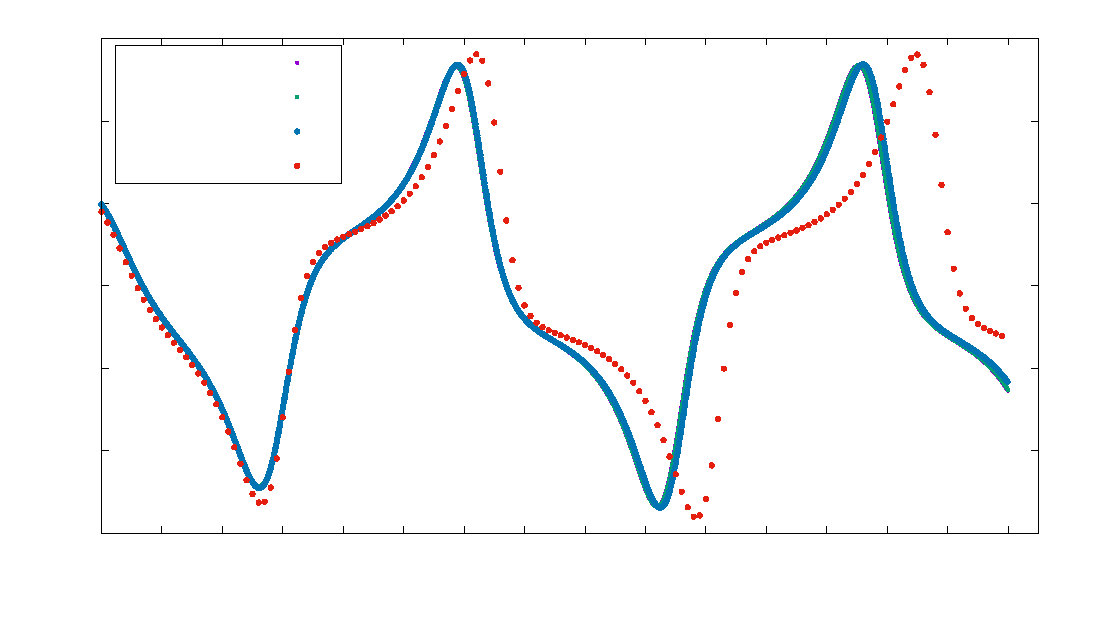
\includegraphics[width={510.20bp},height={283.40bp}]{ConfrP}}%
    \gplfronttext
  \end{picture}%
\endgroup

\end{figure}
e vediamo un comportamento molto simile a quanto visto per $x(t)$. 
\begin{figure}[H]
	\centering
	\input{ConfrPZ.tex}
\end{figure}
Infine confrontiamo le traiettorie nello spazio delle fasi:
\begin{figure}[H]
	\centering
	\scalebox{0.9}{\input{ConfrMu1.tex}}
\end{figure}
e vediamo che, nonostante per $\Delta t = 0.1$ la traiettoria sia piuttosto diversa da quella "esatta", per gli altri time step si ottengono delle traiettorie molto simili. \\ \\
A questo punto possiamo anche calcolare l'ordine di accuratezza delle soluzioni come accennato nella sezione precedente. 
Come detto in precedenza per calcolare l'accuratezza di una soluzione numerica di un'equazione differenziale bisogna posizionarsi in uno spazio normato di funzioni e scegliere la norma in modo adeguato, per poi calcolare la distanza tra la soluzione approssimata e quella esatta nella metrica indotta. \\
In questo caso si è scelta la norma
\begin{equation}
	||f(x)|| = \max_x |f(x)|
\end{equation}
che induce la metrica
\begin{equation}
	||f(x) - g(x)|| = \max_x |f(x) - g(x)|
\end{equation} \\
A questo punto possiamo quindi definire la funzione di errore
\begin{equation}
	E(h) = ||v - v_h|| = \max_x |v - v_h| \leq Ch^n
\end{equation}
dove $h$ è il timestep e $n$ è l'ordine di accuratezza. \\ \\
Per le tre soluzioni citate in precedenza è stato calcolato l'errore mediante un codice che calcola la distanza tra le soluzioni $x(t)$, e questo calcolo è stato fatto confrontando i valori di $x$ a parità di valori di $n$. \\
Per le tre soluzioni si sono ottenuti i seguenti errori:
\begin{equation}
	E(h = 0.1) = 2.04 \ \ \ \ \ \ \ \ \ \  E(h = 0.01) = 0.19  \ \ \ \ \ \ \ \ \ \ E(h = 0.001) = 0.017
\end{equation}
e si nota che questi errori sono consistenti con un'accuratezza di ordine $1$, perchè vediamo che se $h$ diminuisce di un ordine di grandezza, l'errore fa lo stesso.
\subsubsection{Confronto sulla rigidità per $\mu = 10$}
Vogliamo ora confrontare di nuovo le soluzioni approssimate, ma prendendo l'equazione con una costante di smorzamento, e quindi una rigidità, dieci vole maggiore. I timestep utilizzati e che mettiamo a confronto sono $h=0.01$, $h=0.001$, $h=0.0001$ e $h=0.00005$. Similmente a prima, confrontando gli andamenti temporali di $x(t)$ vediamo che per $h = 0.00005$ e $h = 0.0001$ otteniamo delle soluzioni quasi completamente sovrapposte, per $h = 0.001$ ovveniamo una soluzione che si discosta leggermente dalle prime due, mentre con $h = 0.01$ otteniamo una soluzione che si discosta enormemente dalle altre, ed è quindi inadeguata a risolvere l'equazione in maniera soddisfacente.
\begin{figure}[H]
	\centering
	% GNUPLOT: LaTeX picture with Postscript
\begingroup
  % Encoding inside the plot.  In the header of your document, this encoding
  % should to defined, e.g., by using
  % \usepackage[cp1252,<other encodings>]{inputenc}
  \inputencoding{cp1252}%
  \makeatletter
  \providecommand\color[2][]{%
    \GenericError{(gnuplot) \space\space\space\@spaces}{%
      Package color not loaded in conjunction with
      terminal option `colourtext'%
    }{See the gnuplot documentation for explanation.%
    }{Either use 'blacktext' in gnuplot or load the package
      color.sty in LaTeX.}%
    \renewcommand\color[2][]{}%
  }%
  \providecommand\includegraphics[2][]{%
    \GenericError{(gnuplot) \space\space\space\@spaces}{%
      Package graphicx or graphics not loaded%
    }{See the gnuplot documentation for explanation.%
    }{The gnuplot epslatex terminal needs graphicx.sty or graphics.sty.}%
    \renewcommand\includegraphics[2][]{}%
  }%
  \providecommand\rotatebox[2]{#2}%
  \@ifundefined{ifGPcolor}{%
    \newif\ifGPcolor
    \GPcolortrue
  }{}%
  \@ifundefined{ifGPblacktext}{%
    \newif\ifGPblacktext
    \GPblacktextfalse
  }{}%
  % define a \g@addto@macro without @ in the name:
  \let\gplgaddtomacro\g@addto@macro
  % define empty templates for all commands taking text:
  \gdef\gplbacktext{}%
  \gdef\gplfronttext{}%
  \makeatother
  \ifGPblacktext
    % no textcolor at all
    \def\colorrgb#1{}%
    \def\colorgray#1{}%
  \else
    % gray or color?
    \ifGPcolor
      \def\colorrgb#1{\color[rgb]{#1}}%
      \def\colorgray#1{\color[gray]{#1}}%
      \expandafter\def\csname LTw\endcsname{\color{white}}%
      \expandafter\def\csname LTb\endcsname{\color{black}}%
      \expandafter\def\csname LTa\endcsname{\color{black}}%
      \expandafter\def\csname LT0\endcsname{\color[rgb]{1,0,0}}%
      \expandafter\def\csname LT1\endcsname{\color[rgb]{0,1,0}}%
      \expandafter\def\csname LT2\endcsname{\color[rgb]{0,0,1}}%
      \expandafter\def\csname LT3\endcsname{\color[rgb]{1,0,1}}%
      \expandafter\def\csname LT4\endcsname{\color[rgb]{0,1,1}}%
      \expandafter\def\csname LT5\endcsname{\color[rgb]{1,1,0}}%
      \expandafter\def\csname LT6\endcsname{\color[rgb]{0,0,0}}%
      \expandafter\def\csname LT7\endcsname{\color[rgb]{1,0.3,0}}%
      \expandafter\def\csname LT8\endcsname{\color[rgb]{0.5,0.5,0.5}}%
    \else
      % gray
      \def\colorrgb#1{\color{black}}%
      \def\colorgray#1{\color[gray]{#1}}%
      \expandafter\def\csname LTw\endcsname{\color{white}}%
      \expandafter\def\csname LTb\endcsname{\color{black}}%
      \expandafter\def\csname LTa\endcsname{\color{black}}%
      \expandafter\def\csname LT0\endcsname{\color{black}}%
      \expandafter\def\csname LT1\endcsname{\color{black}}%
      \expandafter\def\csname LT2\endcsname{\color{black}}%
      \expandafter\def\csname LT3\endcsname{\color{black}}%
      \expandafter\def\csname LT4\endcsname{\color{black}}%
      \expandafter\def\csname LT5\endcsname{\color{black}}%
      \expandafter\def\csname LT6\endcsname{\color{black}}%
      \expandafter\def\csname LT7\endcsname{\color{black}}%
      \expandafter\def\csname LT8\endcsname{\color{black}}%
    \fi
  \fi
    \setlength{\unitlength}{0.0500bp}%
    \ifx\gptboxheight\undefined%
      \newlength{\gptboxheight}%
      \newlength{\gptboxwidth}%
      \newsavebox{\gptboxtext}%
    \fi%
    \setlength{\fboxrule}{0.5pt}%
    \setlength{\fboxsep}{1pt}%
    \definecolor{tbcol}{rgb}{1,1,1}%
\begin{picture}(9070.00,5668.00)%
    \gplgaddtomacro\gplbacktext{%
      \csname LTb\endcsname%%
      \put(946,1178){\makebox(0,0)[r]{\strut{}$-2$}}%
      \put(946,1653){\makebox(0,0)[r]{\strut{}$-1.5$}}%
      \put(946,2127){\makebox(0,0)[r]{\strut{}$-1$}}%
      \put(946,2601){\makebox(0,0)[r]{\strut{}$-0.5$}}%
      \put(946,3076){\makebox(0,0)[r]{\strut{}$0$}}%
      \put(946,3550){\makebox(0,0)[r]{\strut{}$0.5$}}%
      \put(946,4024){\makebox(0,0)[r]{\strut{}$1$}}%
      \put(946,4498){\makebox(0,0)[r]{\strut{}$1.5$}}%
      \put(946,4973){\makebox(0,0)[r]{\strut{}$2$}}%
      \put(1078,484){\makebox(0,0){\strut{}$0$}}%
      \put(1838,484){\makebox(0,0){\strut{}$2.5$}}%
      \put(2597,484){\makebox(0,0){\strut{}$5$}}%
      \put(3357,484){\makebox(0,0){\strut{}$7.5$}}%
      \put(4116,484){\makebox(0,0){\strut{}$10$}}%
      \put(4876,484){\makebox(0,0){\strut{}$12.5$}}%
      \put(5635,484){\makebox(0,0){\strut{}$15$}}%
      \put(6395,484){\makebox(0,0){\strut{}$17.5$}}%
      \put(7154,484){\makebox(0,0){\strut{}$20$}}%
      \put(7914,484){\makebox(0,0){\strut{}$22.5$}}%
      \put(8673,484){\makebox(0,0){\strut{}$25$}}%
    }%
    \gplgaddtomacro\gplfronttext{%
      \csname LTb\endcsname%%
      \put(209,3075){\rotatebox{-270}{\makebox(0,0){\strut{}x(t)}}}%
      \put(4875,154){\makebox(0,0){\strut{}t}}%
      \csname LTb\endcsname%%
      \put(2662,5219){\makebox(0,0)[r]{\strut{}$h = 0.0001$}}%
      \csname LTb\endcsname%%
      \put(2662,4889){\makebox(0,0)[r]{\strut{}$h = 0.001$}}%
      \csname LTb\endcsname%%
      \put(2662,4559){\makebox(0,0)[r]{\strut{}$h = 0.01$}}%
      \csname LTb\endcsname%%
      \put(2662,4229){\makebox(0,0)[r]{\strut{}$h = 0.00005$}}%
    }%
    \gplbacktext
    \put(0,0){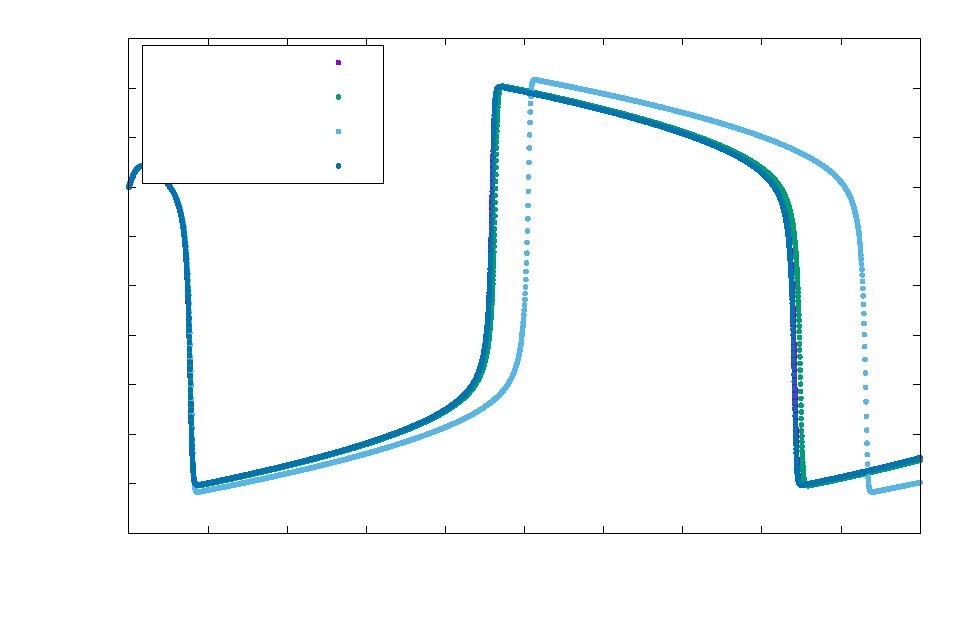
\includegraphics[width={453.50bp},height={283.40bp}]{Comp10X}}%
    \gplfronttext
  \end{picture}%
\endgroup

\end{figure}
Se ora zoomiamo in una piccola regione del grafico vediamo che effettivamente la curva viola e quella blu, corrispondenti a $h = 0.0001$ e $h = 0.00005$ sono quasi indistinguibili. 
\begin{figure}[H]
	\centering
	% GNUPLOT: LaTeX picture with Postscript
\begingroup
  % Encoding inside the plot.  In the header of your document, this encoding
  % should to defined, e.g., by using
  % \usepackage[cp1252,<other encodings>]{inputenc}
  \inputencoding{cp1252}%
  \makeatletter
  \providecommand\color[2][]{%
    \GenericError{(gnuplot) \space\space\space\@spaces}{%
      Package color not loaded in conjunction with
      terminal option `colourtext'%
    }{See the gnuplot documentation for explanation.%
    }{Either use 'blacktext' in gnuplot or load the package
      color.sty in LaTeX.}%
    \renewcommand\color[2][]{}%
  }%
  \providecommand\includegraphics[2][]{%
    \GenericError{(gnuplot) \space\space\space\@spaces}{%
      Package graphicx or graphics not loaded%
    }{See the gnuplot documentation for explanation.%
    }{The gnuplot epslatex terminal needs graphicx.sty or graphics.sty.}%
    \renewcommand\includegraphics[2][]{}%
  }%
  \providecommand\rotatebox[2]{#2}%
  \@ifundefined{ifGPcolor}{%
    \newif\ifGPcolor
    \GPcolortrue
  }{}%
  \@ifundefined{ifGPblacktext}{%
    \newif\ifGPblacktext
    \GPblacktextfalse
  }{}%
  % define a \g@addto@macro without @ in the name:
  \let\gplgaddtomacro\g@addto@macro
  % define empty templates for all commands taking text:
  \gdef\gplbacktext{}%
  \gdef\gplfronttext{}%
  \makeatother
  \ifGPblacktext
    % no textcolor at all
    \def\colorrgb#1{}%
    \def\colorgray#1{}%
  \else
    % gray or color?
    \ifGPcolor
      \def\colorrgb#1{\color[rgb]{#1}}%
      \def\colorgray#1{\color[gray]{#1}}%
      \expandafter\def\csname LTw\endcsname{\color{white}}%
      \expandafter\def\csname LTb\endcsname{\color{black}}%
      \expandafter\def\csname LTa\endcsname{\color{black}}%
      \expandafter\def\csname LT0\endcsname{\color[rgb]{1,0,0}}%
      \expandafter\def\csname LT1\endcsname{\color[rgb]{0,1,0}}%
      \expandafter\def\csname LT2\endcsname{\color[rgb]{0,0,1}}%
      \expandafter\def\csname LT3\endcsname{\color[rgb]{1,0,1}}%
      \expandafter\def\csname LT4\endcsname{\color[rgb]{0,1,1}}%
      \expandafter\def\csname LT5\endcsname{\color[rgb]{1,1,0}}%
      \expandafter\def\csname LT6\endcsname{\color[rgb]{0,0,0}}%
      \expandafter\def\csname LT7\endcsname{\color[rgb]{1,0.3,0}}%
      \expandafter\def\csname LT8\endcsname{\color[rgb]{0.5,0.5,0.5}}%
    \else
      % gray
      \def\colorrgb#1{\color{black}}%
      \def\colorgray#1{\color[gray]{#1}}%
      \expandafter\def\csname LTw\endcsname{\color{white}}%
      \expandafter\def\csname LTb\endcsname{\color{black}}%
      \expandafter\def\csname LTa\endcsname{\color{black}}%
      \expandafter\def\csname LT0\endcsname{\color{black}}%
      \expandafter\def\csname LT1\endcsname{\color{black}}%
      \expandafter\def\csname LT2\endcsname{\color{black}}%
      \expandafter\def\csname LT3\endcsname{\color{black}}%
      \expandafter\def\csname LT4\endcsname{\color{black}}%
      \expandafter\def\csname LT5\endcsname{\color{black}}%
      \expandafter\def\csname LT6\endcsname{\color{black}}%
      \expandafter\def\csname LT7\endcsname{\color{black}}%
      \expandafter\def\csname LT8\endcsname{\color{black}}%
    \fi
  \fi
    \setlength{\unitlength}{0.0500bp}%
    \ifx\gptboxheight\undefined%
      \newlength{\gptboxheight}%
      \newlength{\gptboxwidth}%
      \newsavebox{\gptboxtext}%
    \fi%
    \setlength{\fboxrule}{0.5pt}%
    \setlength{\fboxsep}{1pt}%
    \definecolor{tbcol}{rgb}{1,1,1}%
\begin{picture}(9070.00,5668.00)%
    \gplgaddtomacro\gplbacktext{%
      \csname LTb\endcsname%%
      \put(814,704){\makebox(0,0)[r]{\strut{}$1$}}%
      \put(814,2680){\makebox(0,0)[r]{\strut{}$1.5$}}%
      \put(814,4657){\makebox(0,0)[r]{\strut{}$2$}}%
      \put(2234,484){\makebox(0,0){\strut{}$12.5$}}%
      \put(4380,484){\makebox(0,0){\strut{}$15$}}%
      \put(6527,484){\makebox(0,0){\strut{}$17.5$}}%
      \put(8673,484){\makebox(0,0){\strut{}$20$}}%
    }%
    \gplgaddtomacro\gplfronttext{%
      \csname LTb\endcsname%%
      \put(209,3075){\rotatebox{-270}{\makebox(0,0){\strut{}x(t)}}}%
      \put(4809,154){\makebox(0,0){\strut{}t}}%
      \csname LTb\endcsname%%
      \put(7686,5219){\makebox(0,0)[r]{\strut{}$h = 0.0001$}}%
      \csname LTb\endcsname%%
      \put(7686,4889){\makebox(0,0)[r]{\strut{}$h = 0.001$}}%
      \csname LTb\endcsname%%
      \put(7686,4559){\makebox(0,0)[r]{\strut{}$h = 0.01$}}%
      \csname LTb\endcsname%%
      \put(7686,4229){\makebox(0,0)[r]{\strut{}$h = 0.00005$}}%
    }%
    \gplbacktext
    \put(0,0){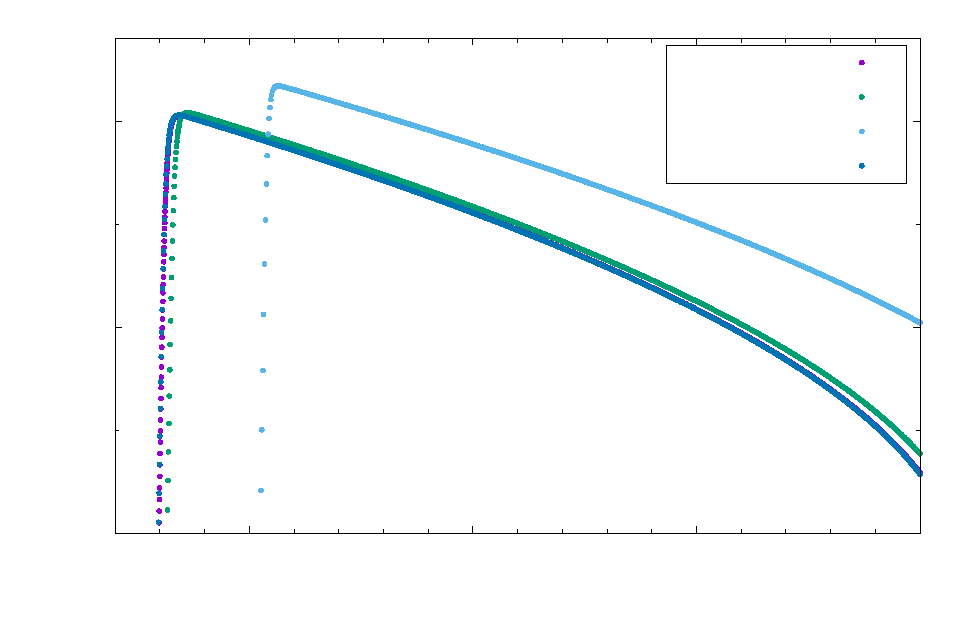
\includegraphics[width={453.50bp},height={283.40bp}]{Comp10XZ}}%
    \gplfronttext
  \end{picture}%
\endgroup

\end{figure}
Ora effettuamiamo lo stesso confronto per gli andamenti temporali degli impulsi $p(t)$
e vediamo che valgono le stesse considerazioni appena fatte per l'andamento di $x(t)$. 
\begin{figure}[H]
	\centering
	\input{Comp10PZ.tex}
\end{figure}
Se come prima effettuiamo uno zoom vediamo che le curve con $h = 0.0001$ e $h = 0.00005$ sono quasi indistinguibili.
\begin{figure}[H]
	\centering
	% GNUPLOT: LaTeX picture with Postscript
\begingroup
  % Encoding inside the plot.  In the header of your document, this encoding
  % should to defined, e.g., by using
  % \usepackage[cp1252,<other encodings>]{inputenc}
  \inputencoding{cp1252}%
  \makeatletter
  \providecommand\color[2][]{%
    \GenericError{(gnuplot) \space\space\space\@spaces}{%
      Package color not loaded in conjunction with
      terminal option `colourtext'%
    }{See the gnuplot documentation for explanation.%
    }{Either use 'blacktext' in gnuplot or load the package
      color.sty in LaTeX.}%
    \renewcommand\color[2][]{}%
  }%
  \providecommand\includegraphics[2][]{%
    \GenericError{(gnuplot) \space\space\space\@spaces}{%
      Package graphicx or graphics not loaded%
    }{See the gnuplot documentation for explanation.%
    }{The gnuplot epslatex terminal needs graphicx.sty or graphics.sty.}%
    \renewcommand\includegraphics[2][]{}%
  }%
  \providecommand\rotatebox[2]{#2}%
  \@ifundefined{ifGPcolor}{%
    \newif\ifGPcolor
    \GPcolortrue
  }{}%
  \@ifundefined{ifGPblacktext}{%
    \newif\ifGPblacktext
    \GPblacktextfalse
  }{}%
  % define a \g@addto@macro without @ in the name:
  \let\gplgaddtomacro\g@addto@macro
  % define empty templates for all commands taking text:
  \gdef\gplbacktext{}%
  \gdef\gplfronttext{}%
  \makeatother
  \ifGPblacktext
    % no textcolor at all
    \def\colorrgb#1{}%
    \def\colorgray#1{}%
  \else
    % gray or color?
    \ifGPcolor
      \def\colorrgb#1{\color[rgb]{#1}}%
      \def\colorgray#1{\color[gray]{#1}}%
      \expandafter\def\csname LTw\endcsname{\color{white}}%
      \expandafter\def\csname LTb\endcsname{\color{black}}%
      \expandafter\def\csname LTa\endcsname{\color{black}}%
      \expandafter\def\csname LT0\endcsname{\color[rgb]{1,0,0}}%
      \expandafter\def\csname LT1\endcsname{\color[rgb]{0,1,0}}%
      \expandafter\def\csname LT2\endcsname{\color[rgb]{0,0,1}}%
      \expandafter\def\csname LT3\endcsname{\color[rgb]{1,0,1}}%
      \expandafter\def\csname LT4\endcsname{\color[rgb]{0,1,1}}%
      \expandafter\def\csname LT5\endcsname{\color[rgb]{1,1,0}}%
      \expandafter\def\csname LT6\endcsname{\color[rgb]{0,0,0}}%
      \expandafter\def\csname LT7\endcsname{\color[rgb]{1,0.3,0}}%
      \expandafter\def\csname LT8\endcsname{\color[rgb]{0.5,0.5,0.5}}%
    \else
      % gray
      \def\colorrgb#1{\color{black}}%
      \def\colorgray#1{\color[gray]{#1}}%
      \expandafter\def\csname LTw\endcsname{\color{white}}%
      \expandafter\def\csname LTb\endcsname{\color{black}}%
      \expandafter\def\csname LTa\endcsname{\color{black}}%
      \expandafter\def\csname LT0\endcsname{\color{black}}%
      \expandafter\def\csname LT1\endcsname{\color{black}}%
      \expandafter\def\csname LT2\endcsname{\color{black}}%
      \expandafter\def\csname LT3\endcsname{\color{black}}%
      \expandafter\def\csname LT4\endcsname{\color{black}}%
      \expandafter\def\csname LT5\endcsname{\color{black}}%
      \expandafter\def\csname LT6\endcsname{\color{black}}%
      \expandafter\def\csname LT7\endcsname{\color{black}}%
      \expandafter\def\csname LT8\endcsname{\color{black}}%
    \fi
  \fi
    \setlength{\unitlength}{0.0500bp}%
    \ifx\gptboxheight\undefined%
      \newlength{\gptboxheight}%
      \newlength{\gptboxwidth}%
      \newsavebox{\gptboxtext}%
    \fi%
    \setlength{\fboxrule}{0.5pt}%
    \setlength{\fboxsep}{1pt}%
    \definecolor{tbcol}{rgb}{1,1,1}%
\begin{picture}(10204.00,5668.00)%
    \gplgaddtomacro\gplbacktext{%
      \csname LTb\endcsname%%
      \put(682,1000){\makebox(0,0)[r]{\strut{}$0$}}%
      \put(682,2483){\makebox(0,0)[r]{\strut{}$5$}}%
      \put(682,3965){\makebox(0,0)[r]{\strut{}$10$}}%
      \put(682,5447){\makebox(0,0)[r]{\strut{}$15$}}%
      \put(814,484){\makebox(0,0){\strut{}$10$}}%
      \put(2313,484){\makebox(0,0){\strut{}$10.5$}}%
      \put(3812,484){\makebox(0,0){\strut{}$11$}}%
      \put(5311,484){\makebox(0,0){\strut{}$11.5$}}%
      \put(6809,484){\makebox(0,0){\strut{}$12$}}%
      \put(8308,484){\makebox(0,0){\strut{}$12.5$}}%
      \put(9807,484){\makebox(0,0){\strut{}$13$}}%
    }%
    \gplgaddtomacro\gplfronttext{%
      \csname LTb\endcsname%%
      \put(209,3075){\rotatebox{-270}{\makebox(0,0){\strut{}x(t)}}}%
      \put(5310,154){\makebox(0,0){\strut{}t}}%
      \csname LTb\endcsname%%
      \put(2398,5219){\makebox(0,0)[r]{\strut{}$h = 0.0001$}}%
      \csname LTb\endcsname%%
      \put(2398,4889){\makebox(0,0)[r]{\strut{}$h = 0.001$}}%
      \csname LTb\endcsname%%
      \put(2398,4559){\makebox(0,0)[r]{\strut{}$h = 0.01$}}%
      \csname LTb\endcsname%%
      \put(2398,4229){\makebox(0,0)[r]{\strut{}$h = 0.00005$}}%
    }%
    \gplbacktext
    \put(0,0){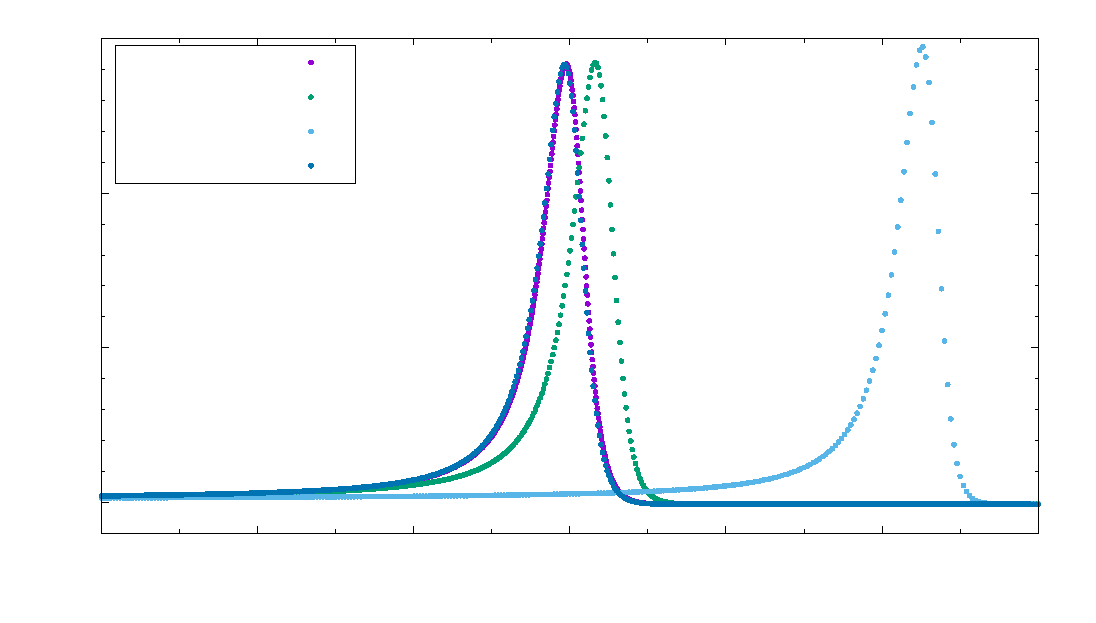
\includegraphics[width={510.20bp},height={283.40bp}]{Comp10PZZ}}%
    \gplfronttext
  \end{picture}%
\endgroup

\end{figure}
Infine confrontiamo le traiettorie nello spazio delle fasi:
\begin{figure}[H]
	\centering
	\input{Comp10.tex}
\end{figure}
Alla luce dei confronti che abbiamo appena fatto capiamo che, come atteso, il fatto che la costante di smorzamento, che in questo caso indica anche la rigidità dell'equazione, sia di un'ordine di grandezza più grande richiede anche che i timestep siano un ordine di grandezza più piccoli. Infatti, il timestep "h = 0.1", che con $\mu = 1$ dava risultati approssimativi ma comunque accettabili, con $\mu=10$ è assolutamente insufficiente e presenta lo stesso comportamento che si otteneva usando un timestep $h = 1$ con $\mu = 1$. 
\section{Circuito elettronico}
Per realizzare un circuito che descriva l'equazione di Van Der Pol sono necessari elementi circuitali attivi che appbiano proprietà cubiche non lineare della forma
\begin{equation}
	i = \phi(v) = \gamma V^3 - \alpha V
\end{equation}
dove $i$ è la corrente e $V$ è il voltaggio. \\
In origine Van Der Pol creò il circuito utilizzando una valvola termoionica, o tubo a vuoto, ma dopo l'invenzione del diodo a tunnel è divenuto molto più facile realizzare circuiti di questo tipo. \\
Mediante l'utilizzo di un diodo a tunnel che abbia la caratteristica I-V
\begin{equation}
	i = \phi_t(V) = \phi(V - E_0) + i_0
\end{equation}
l'equazione del circuito prende la forma
\begin{equation}
	\begin{cases}
		\dot{V} = \dfrac{1}{C}\left(-\phi(V) - W\right) \\
		\dot{W} = \dfrac{1}{L}V
	\end{cases} 
\end{equation}
e combinando le due equazioni di questo sistema si ottiene l'equazione differenziale
\begin{equation}
	\ddot{V}-\frac{1}{C}\left( \alpha - 3\gamma  V^2\right)\dot{V} + \frac{1}{LC} = 0
\end{equation}
che è proprio l'equazione di Van Der Pol. Guardando bene l'equazione infatti si vede che l'ultimo termine è proprio il termine oscillativo di un circuito LC, che va a formare un oscillatore armonico elettronico di pulsazione $\omega = 1/\sqrt{LC}$. Il termine di mezzo invece è molto semplicemente riconoscibile come il termine dissipativo non lineare caratteristico dell'oscillatore di Van Der Pol. \\ \\
Quando la costante di smorzamento $\mu$ è grande, il periodo di oscillazione dell'oscillatore è proporzionale a $\mu$, quindi il sistema ha periodo di oscillazione $T \propto \mu\sqrt{LC} = L\alpha$. Dal momento che $\alpha$ equivale all'inverso di una resistenza, si ottiene $T \propto L/r$. Il rapporto $L/R$ è la costante del tempo di rilassamento nei circuiti LR, e questo giustifica il nome "relaxation-oscillation". 
\section{Appendice}
\section{Bibliografia}
1) "Modelling complex systems" \\
2) Esponenziale rambaldi \\
3) Oscillatore rambaldi \\
4) Wikipedia \\
5) Scholarpedia \\


\end{document}